\documentclass[conference]{IEEEtran}
%\setlength{\parskip}{0.25cm plus2mm minus1mm}
\usepackage{float} % positions of tables and figures
\usepackage{graphicx} % pic
\usepackage{amsmath} % math
\usepackage{amssymb}
\usepackage{url}
 %\usepackage{hyperref} 
 %\hypersetup{breaklinks} 
 \usepackage{listings}
\usepackage{color}

\definecolor{dkgreen}{rgb}{0,0.6,0}
\definecolor{gray}{rgb}{0.5,0.5,0.5}
\definecolor{mauve}{rgb}{0.58,0,0.82}

\lstset{frame=tb,
  language=Java,
  aboveskip=3mm,
  belowskip=3mm,
  showstringspaces=false,
  columns=flexible,
  basicstyle={\small\ttfamily},
  numbers=none,
  numberstyle=\tiny\color{gray},
  keywordstyle=\color{blue},
  commentstyle=\color{dkgreen},
  stringstyle=\color{mauve},
  breaklines=true,
  breakatwhitespace=true
  tabsize=3
}

\newcommand{\squishlist}{
 \begin{list}{$\bullet$}
  { \setlength{\itemsep}{0pt}
     \setlength{\parsep}{3pt}
     \setlength{\topsep}{3pt}
     \setlength{\partopsep}{0pt}
     \setlength{\leftmargin}{1.5em}
     \setlength{\labelwidth}{1em}
     \setlength{\labelsep}{0.5em} } }

\newcommand{\squishlisttwo}{
 \begin{list}{$\bullet$}
  { \setlength{\itemsep}{0pt}
     \setlength{\parsep}{0pt}
    \setlength{\topsep}{0pt}
    \setlength{\partopsep}{0pt}
    \setlength{\leftmargin}{2em}
    \setlength{\labelwidth}{1.5em}
    \setlength{\labelsep}{0.5em} } }

\newcommand{\squishend}{
  \end{list}  }
  
\begin{document}
\title{Quality Metrics of Test Suites in Test-Driven Designed Applications}

\author{
\IEEEauthorblockN{Hessah Alkaoud}
\IEEEauthorblockA{Department of Computer Science\\
University of Colorado at Colorado Springs, USA\\
Email: halkaoud@gmail.com}
\and
\IEEEauthorblockN{Kristen Walcott-Justice}
\IEEEauthorblockA{Department of Computer Science\\
University of Colorado at Colorado Springs, USA\\
Email: kjustice@uccs.edu}
}
%\date{\today}
\maketitle
\begin{abstract}
%smooth this all out: 
As software engineering methodologies continue to progress, new techniques for writing and developing software have evolved. One of these methods is known as Test-Driven Development (TDD). In TDD, tests are written first, prior to code development, aiding in both maintenance and software evolution efforts.  The principle of TDD dictate that a developer should not write a code without first having a test to execute it.  Thus, in terms of code coverage, the quality of test suites written using TDD  is likely to be high.  However, it is unclear if test suites developed using TDD exhibit high quality in terms of other metrics such as mutation score.  Moreover, the association between coverage and mutation score is little studied.Also, scientifically grounded empirical evidence still very limited.

the paper empirically analyzes real-world applications written using TDD and more traditional techniques.  Specifically, we demonstrate the quality of the associated test suites based on two quality metrics: 1) structure-based criterion represented by branch coverage and statement coverage, 2) fault-based criterion represented by mutation scores. We learn that test suites with high branch test coverage will also have high mutation scores, and we especially reveal this in the case of TDD applications. the results reveal that Test-Driven Development is an effective approach that improves the quality of the test suite to cover more of the source code and also to reveal more faults based on mutation analysis.%KJ- results should go here. %Greg- comment on the size of the programs and test suites
 
\end{abstract}
%\keywords { Test Driven Development , Test experimentation, Measurement, quality metrics, Mutation Score}

\section{Introduction}
%In software engineering, writing tests is vital to the development and maintenance processes (in the paragraph, write that and expand on why testing is important)
In software engineering, writing tests is vital to the development and maintenance processes because it verifies the correctness of the implementation of the software through program execution and analysis. During development, testing is a way to verify the completeness of the requirements.  Testing also helps to ensure that the software has achieved an appropriate level of quality. In the maintenance phase and software evolution, software testing is important when adding new functionality or refactoring to check the correctness of the changes. Moreover, testing is vital to verify that new features do not cause the program to regress.  Due to this importance, new methods of developing programs and tests together have been devised to improve the evolution of software systems.  One of these techniques is known as Test-Driven Development TDD. Practices of TDD require that tests be written prior to the writing of code.  In this methodology, no code should be written without first having at least one test case to cover such code.  Thus, the quality of the code as measured using coverage should be high for TDD applications.  However, there is little research in comparing the code coverage of such applications to other code quality metrics. 

%Writing tests is challenging. Some just write them after the code is done, others write tests after code, or, in a new technique, tests are written prior to any code. This is called TDD- explain
Traditionally, tests are written in an ad-hoc fashion by the developers after the code is completed or in tandem with development by a quality assurance QA team.  In TDD, however, tests are written prior to any code.  The TDD process is also known as test-first or red-green-refactoring. Today TDD is being widely adopted in industry, including large software firms such as Microsoft and IBM~\cite{nagappan2008realizing}.   TDD has also gained in popularity with the introduction of the eXtreme Programming XP methodology~\cite{beck2004extreme}, and it is sometimes used as a stand-alone approach for software engineering maintenance tasks such as adding features to legacy code~\cite{feathers2004working}. In TDD, the software is often developed in short iterative cycles and in each cycle, testing is repeated for each testable component of the program. The pattern of the cycles can be explained as the following:
\squishlist 
\item Write the test and run it to see that it fails.
\item If the test fails, implement the code that will cause the test to run and pass the test.
\item Refactor the design of both the test and the code. 
\squishend
Refactoring is a process of altering the code for the purpose of enhancing its design, readability, maintainability \ldots without violating existing code functionality~\cite{fowler1999refactoring}.

%Once a test suite is written, it's also important to evaluate that test suite-- how can we evaluate?
Once a test suite is written and complete, it is also important to evaluate the quality of the test suite. Many program-based adequacy criterion have been developed to determine whether or not a test suite adequately tests the application~\cite{weyuker1988evaluation}. Program-based adequacy criterion exploit both structure-base criteria and fault-based criteria. A structure-based criterion requires the creation of a test suite that solely requires the exercising of certain control structures and variables within program~\cite{kapfhammer-testing-handbook}. Fault-based test adequacy criteria, on the other hand, attempt to ensure that the program does not contain the types of faults that are commonly introduced into software systems by programmers~\cite{demillo1978hints, zhu1997software}.  One of the most common types of test quality evaluation in both industry and academic work is based on structurally-based criterion which is commonly analyzed in terms of statement or branch coverage~\cite{weyuker1988evaluation}.

%TDD plus evaluation? Coverage should be high- explain why. But is the suite good?
When developing programs using TDD, code is only written when a test shows that it is needed.  In theory, no production code in TDD should be developed unless it has at least one associated test. Therefore, by nature, the code coverage of TDD-based tests should be high for their associated applications. Both the literature and practice indicate that the use of TDD yields several benefits. For instance, TDD leads to improved test coverage~\cite{astels2003test}. However,  statement coverage and branch coverage have been shown to not necessarily give firm evidence of high-quality test suites~\cite{zhu1997software}.% Greg: Suggested another paper to cite here. 
%~\cite{}.% statement coverage is so weak because even some control transfers may be missed from an adequate tes \cite{zhu1997software}  %Other ways of evaluating quality- Coverage is traditional, but mutation (what is that in one sentence?) can also help
%Other ways of evaluating quality- Coverage is traditional, but mutation which is a fault-based technique can also help.

In recent years, mutation testing have been used as another method for evaluating test suite quality. Mutation testing is a fault-based which measures the fault-finding effectiveness of test suites on the basis of induced faults~\cite{demillo1978hints, hamlet1977testing}. Mutation testing is a well-known technique to design a new software tests or to evaluate the quality of existing software tests and test suites. The idea of using mutants to measure test suite adequacy was originally proposed by DeMillo et al.~\cite{demillo1978hints}. Mutation testing involves seeding faults in the source program. Each altered version of the source is called a mutant. When a test reveals the mutant then the mutant said to be killed. % Greg: Commented that we might need to eaplain better how test reveal the mutatnts.
The ratio of killed mutants/generated mutants is known as the mutation score. In mutation testing, in a simple statement such as  \texttt{if (a < b)}, the \texttt{<} sign will be replaced with all other possible relational operators such as \texttt{>, <=, >= , ==, !=}. 
%The use of mutation operators yields results in the empirical assessment of quality for current testing techniques~\cite{andrews2005mutation}. % Greg: Commented that he cannot aundestand the meaining of this sentence.

%Given the rise in popularity of TDD approaches, a question is whether TDD actually promotes high quality test suites or not? In this work, we....
Given the rise in popularity of TDD approaches, the question is whether TDD actually promotes high-quality test suites or not? In this paper, we  investigate if TDD methodology promotes higher test suite quality than traditional test design approaches. To show this, we analyze and compare three quality metrics: branch coverage, statement coverage, and mutation score when applied to two sets of programs: programs that were designed using the TDD methodology and programs designed using standard testing techniques. In this paper, we use the term \textit{standard testing technique} to refer to any tests that were developed using methodologies that are not TDD oriented. We first analyze the size and complexity of the programs.  Then we investigate the statement and branch coverage quality of the existing test suites. Next, we apply a mutation testing tool to determine the mutation score of the test suite.  Finally, we analyze the association between test coverage and mutation scores in estimating overall test suite quality.

%KJ- What we learn paragraph needed-- needs improving     %HESSAH: NEED TO REVISE THIS FOR NEW RESULTS

Our results show that test-driven development is significantly different from the other development approaches on mutation score. We demonstrate a relationship between the mutation score and traditional coverage metrics, statement coverage and branch coverage, and that the correlation with branch coverage is stronger. A 54\% of the programs reflects a relationship with statement coverage and more as %Greg: rephrase
62\% reflects a relation with branch coverage. % KJ Do we need numbers here? is that enough?

In summary, the main contributions of this research are as follows:
\squishlist  
\item An empirical analysis of test suites developed using TDD for open-source applications.
\item An empirical analysis of test suites developed using other non-TDD methodology for open-source applications.
\item An examination of the positive effect of TDD on the quality of software tests based on two quality metrics, code coverage and mutation score.
\item A comparison of test suites that are developed using TDD to the other that are developed not using TDD.
\item An initial study of the relationship phenomena between the two test suite quality metrics of TDD applications.
%\item A discussion of the observed trends.
\squishend
% Greg: Connect these to specific sections of the paper

\section{Related Work} \label{sec:relatedWork}
%TDD is a subject for many researchers. TDD techniques have been addressed from many angles. Most of them revolve around three topics: internal quality, external quality and productivity.

There always has been trade-off between level of control and degree of realism. ``the realistic situation is often complex and non-deterministic, which hinders the understanding of what is happening, especially for studies with explanatory purposes. On the other hand, increasing the control reduces the degree of realism, sometimes leading to the real influential factors being set outside the scope of the study.''\cite{runeson2009guidelines} %(Preface)
 
With regard to code coverage and/or mutation score, we have found five controlled experiments (e.g. \cite{george2004structured}, \cite{madeyski2010impact}, and \cite{panvcur2011impact}) and only one of case study \cite{bhat2006evaluating} and another one controlled case study \cite{siniaalto2007comparative}. (Statistics of both research types in TDD context) . In Table: 1, we list all the collected publication and we classify them based on: type of experiment (e.g. controlled, case study, or controlled case study), How many TDD projects are studied, how many non-TDD projects, maximum line of code LOC for the studied projects, type of coverage metrics used, and an indicator if mutation score have been used. Coverage metrics was studied in 5 papers while mutation score metrics only recently introduced in 2 latest papers. Researchers reported higher ( e.g.\cite{siniaalto2007comparative} \cite{bhat2006evaluating}), similar(e.g. \cite{madeyski2010impact}) or slightly lower \cite{geras2004prototype} code coverage as a result of the Test-driven development TDD or alternatively called Test First TF practice.  While studying the mutation score indicator didn’t find significant different between the two approaches. With total respect to controlled experiment, we notice that the positive impact of TDD seems to be more obvious when not using controlled experiment \cite{bhat2006evaluating} \cite{siniaalto2007comparative}. 

\begin{table*}[htbp]
\caption{Summery of the previous studies}
\label{table:relateWork}
\centering
%\begin{tabular}{l l r l r l l l p{1in}}
\begin{tabular}{p{0.5in} p{0.5in} p{0.25in} p{0.25in} p{0.75in} p{0.5in} p{3in} p{1in} p{1in}}
\hline
\textbf{Publication} & \textbf{Type } & \textbf{TDD LOC} & \textbf{Non-TDD LOC} & \textbf{Type of Coverage metrics} & \textbf{Mutation testing?} & \textbf{Description } \\ \hline
\cite{siniaalto2007comparative} & controlled case study & \multicolumn{1}{r}{5800} & \(>\) 7700 & Method, statement, and branch coverage  & - & Compared 2 iterative test-last projects to 1 TDD project. All the results were significantly better in the project that employed TDD. In the two iterative projects, the test classes were implemented, they were not as thorough as the ones implemented in TDD project \\ \\
\cite{janzen2006influence} & Controlled experiment   & \(>\)1053 & \(>\)995 & Statement and branch coverage & - & Compare an identical project among three development teams: TDD, iterative test-last development, and manual testing developed after the implementation phase. Results of code coverage indicates that the test coverage was relatively low regardless of the development approach \\ \\
\cite{bhat2006evaluating} & Case study & \multicolumn{1}{r}{49200} & \multicolumn{1}{r}{10000} & Block coverage & - & Compared the impacts of TDD and non-TDD development processes of two industrial case studies conducted at Microsoft. The block coverage was 79–88 \% at unit test level in projects employing TDD giving and indications that that TDD may improve test coverage. \\ \\ 
\cite{george2004structured} & controlled experimental & \multicolumn{1}{r}{200} & \multicolumn{1}{r}{200} & Method, statement, and branch coverage  & - & Compared TDD with the conventional test-last development and reported that TDD test cases achieved a mean of 98 \% method, 92 \% statement and 97 \% branch coverage \\ \\ 
\cite{pancur2003towards} & controlled experiment & n/a & n/a & Method, statement, and branch coverage & - & Studies TDD and iterative test-last development on 38 senior students and their results of their comparison did not show any significant differences between them. \\ \\ 
\cite{flohr2006lessons} & controlled experiment & n/a & n/a & Method, statement, and branch coverage & - & Compared investigate the impact of test-first compared to a classical-testing approach and found little or no significant difference in terms of code coverage.  \\ \\
\cite{geras2004prototype} & Controlled experiment  & n/a & n/a & Branch coverage & - & There were no differences in term of code coverage; the branch coverage for every submitted program was more than 95\%, except one participant’s programs that didn’t run at all. \\ \\
\cite{madeyski2010impact} & controlled experiment &  &  & Branch coverage & yes & No statistical significant difference was found between TDD and TLD team.  \\ \\
\cite{panvcur2011impact} & controlled experiment &  &  & Branch coverage & yes & No statistical difference regarding mutation score indicator.  \\ \hline
\end{tabular}
\end{table*}

Only recently researchers have started to conduct experiments on TDD with the use of  mutation analysis. We will discuss some of these studies and how they pertain to our work. There are three major studies comparing TDD to non-TDD practices and their impacts of code coverage and mutation score. 

Madeyski \cite{madeyski2010impact} (2010) investigated how TDD can impact branch coverage and mutation score indicators. In this experiment, twenty-two third and fourth-year graduate MSc software engineering students were divided in two groups: test-first (TF) and the test- last(TL). The participants were asked to develop a web based conference paper submission system. The main result of this study is ``that the TF programming practice, used instead of the
classic TL technique, does not significantly affect branch coverage and mutation score indicator" \cite{madeyski2010impact}.

Following this work, Pancur and Ciglaric \cite{panvcur2011impact} (2011) conducted a family of controlled experiments comparing test-driven development to iterative test-last development with focus on productivity, code properties (external quality and complexity) and (code coverage and fault-finding capabilities) of tests. In their study, the minimum TDD mutation score was 22.0 and the maximum was 88.8. %which is a wide range that mybe caused by some other factors wasn't under study.
The results of the research state that "the effect of TDD on mutation is small and in the positive direction (based either only on ID2, r = 0.149)" \cite{panvcur2011impact}. %KJ: need to fix...

Finally, Cauevic and Punnekkat \cite{cauevic2012quality} (2012) also measured code coverage and  mutation score indicators. However, those two metrics were utilized for an analysis to external attribute, a defect detecting ability attribute. For each participant's test suite they calculated a total number of defects discovered in all other participants source code. Fourteen participants were randomly grouped in two groups; the first group used test-first development and the second was used as a control (test-last) group. Participants of the test-first group were guided to use TDD to develop software solutions. The task of both groups were to completely implement and test the same project, a bowling game score calculation algorithm. This research and that performed by Madeyski \cite{madeyski2010impact} show similar results, concluding that there are no statistically significant differences in branch coverage and mutation score indicators between the test-first and the test-last groups.  

In each of these papers, only small programs were used, and these were developed within a controlled, academic setting. No industrial-sized programs were considered. Our work expands upon these studies by analyzing industry-level, open source applications. To the best of our knowledge, no studies have been conducted comparing test-first and test-last techniques with regard to final code quality based coverage and mutation score on larger, already produced and in-use applications.
Very few studies, other than the ones mentioned above, have considered the correlation between code coverage and mutation scores for estimating code quality. Andrews et al \cite{andrews2006using} analyzed four common control and data flow testing criteria on middle sized industrial programs with a comprehensive pool of test cases and known faults. However, mutation testing and mutation score are not considered. Fraser and Zeller \cite{fraser2012mutation} present an automated approach to generate unit tests that detect mutations for object-oriented classes. While their tool, $\mu$test, does produce tests with strong fault-finding ability, there is no link back to how mutants relate to less expensive, code coverage-based analyses. 

\section{TDD Practices}\label{sec:TDDPractices}
Test-driven development is a software development process that is based on repeating a very short development cycle. There are several variations of test-driven development, although the main method is called Test-First or testing via a red-green-refactoring cycle. Refactoring is a process of altering the code for the purpose of enhancing its design, readability, maintainability, etc. without violating existing code functionality \cite{fowler1999refactoring}. %of the most prominent, quality related, practices in agile is test driven development.
The TDD process is performed in the following six steps:
%\squishlist 
\begin{enumerate}
\item Add test code for a new functionality or a specific desired improvement.
\item Run the test code and see the test fail (red).
\item Implement the production code according to the test.
\item Run all tests again and make sure they pass (green).
\item Repeat 3, 4 until the test passes.
\item Refactor the production code and the test.
\item Repeat steps 1 through 7 to program development completion.
%\squishend
\end{enumerate}

Test-driven development implies quality benefits to the software. It is true that TDD requires more test-based code than without TDD because of the thoroughness of the unit test code, but the large numbers of tests also contributes to limiting the number of defects in the code and supporting more confidant refactoring. The frequent and early nature of the TDD testing helps to reveal defects early in the development process, reducing the number of bugs that may be observed later in time. Moreover, TDD tests that are written prior to code development and are run repeatedly are more likely to detect any regression of the code's behavior. This allows developers to discover problems that may arise when a later change in the implementation unexpectedly affects other functionality.

In software engineering, behaviour-driven development BDD is another software development process that is built based on test-driven development (TDD). The original developer of BDD, Dan North \cite{north2006introducing}, came up with the notion of BDD because he was dissatisfied with the lack of any specification within TDD of what should be tested and how. Astels notes, ``Behavior-Driven Development is what you were doing already if you're doing Test-Driven Development very well \cite{Astels2006Beyond}.''  In this work, we will use both TDD and BDD applications.

\section{Methodology}\label{sec:Methodology}

\subsection{selection of programs}
	There are a number of challenges in selecting such applications.  Many open source projects are not well tested. Also, how to recognize TDD applications.
    
    The case study are executed on Java language open source projects. In our work, we focus on a set of open source projects that are often used in software engineering research, the SF100~\cite{bench_sf100}, as well as several frequently used programs from Apache Commons. The SF100 is a set of 100 open source Java projects selected from SourceForge. We also considered programs that are known to be developed using TDD ~\cite{mlevinson:2008}. 

\subsection{Measuring code coverage}
Code coverage metrics are common for evaluating the quality of test suites. Coverage metrics check how many elements of the source code  have been \textit{executed} by the test. Code coverage falls under structurally-based criterion that requires the creation of a test suite that solely requires the exercising of certain control structures, statements, or variables within the program\cite{kapfhammer-testing-handbook}. There are many coverage metrics types that have been used and proposed, some of which include statement coverage, branch coverage, and condition coverage. Branch coverage criteria and statement coverage criteria are the two most popular examples of structural adequacy criteria that are used in existing coverage analysis tools and by industry\cite{weyuker1988evaluation}.

Statement Coverage metrics require executing each statement in the program at least once during testing, in other word is the coverage of all nodes in the flow graph \cite{zhu1997software}.

Branch Coverage metrics require the execution of each control transfer (true,false) of each branch (e.g. if statements, loops)  in the program under test at least once, or the coverage of all edges in the flow graph \cite{zhu1997software}.\\

To distinguish the differences between statement and branch coverage, consider the following code:
\begin{lstlisting}
public int returnInput(int input, boolean condition1, boolean condition2, boolean condition3) {
  int x = input;
  int y = 0;
  if (condition1) 
    x++;
  if (condition2) 
    x--;
  if (condition3) 
    y=x;
  return y;
\end{lstlisting}
with the following associated test case:\\
\textbf{Test 1:} \texttt{\small 
shouldReturnInput(x, true, true, true)}


In this case, statement coverage would be 100\% as every statement would be executed.  Test case 1 will guarantee that each statement in the code will be exercised. However, the branch coverage is only 50\% because branch coverage requires checking that both edges of each branch execute.  To improve the branch coverage to 100\%, a second test case could be added as follows:\\ 
\textbf{Test 2:} \texttt{\small 
shouldReturnInput(x, false, false, false)}

From these examples of test cases, we observe that branch coverage implies statement coverage, because exercising every branch leads to executing every statement~\cite{steve2011Code}. Branch coverage is a good indicator of test quality, but still branch coverage is not enough to truly estimate test quality because it does not imply the execution of all possible paths. Consider the following example: This simple method has two tests, and the branch coverage calculation reports 100\% branch coverage even though there is no test to catch when \texttt{i ==0}.\\
%Greg: {i==0} the specifiying is not consistent
\begin{lstlisting}
public static String foo(int i) {
  if ( i <= 0 ) {
      return "foo"; 
  } else {
      return "bar";
  }
}
@Test
public void shouldReturnBarWhenGiven1() {
  assertEquals("bar", foo(1));
}
@Test
public void shouldReturnFooWhenGivenMinus1() {
  assertEquals("foo", foo(-1));
}
\end{lstlisting}
Therefore, high code coverage does not necessarily imply full coverage and thorough testing overall. 
% Greg: suggested paper to cite for Wey uker, Frankl, and Wong 
% Not this: "All-uses vs mutation testing: An experimental comparison of effectiveness" frank
% not even this "Mutation versus All-uses: An Empirical Evaluation of Cost, Strength and Effectiveness " W. Eric Wong

\subsection{Measuring mutation Score}
Mutation analysis is an alternative approach for determining code quality. Mutation analysis was originally introduced in~\cite{demillo1978hints,budd1980mutation}. Mutation testing is a fault-based technique which measures the fault-finding effectiveness of test suites on the basis of introduced faults~\cite{demillo1978hints,hamlet1977testing}. Fault-based test adequacy criterion attempt to ensure that the program does not contain the types of faults that are commonly introduced into software systems by programmers~\cite{demillo1978hints}. Mutation testing involves modifying a program's source code in small ways in order to seed in faults~\cite{offutt1994practical}. Each modified version of the program is called a \textit{mutant}, and each mutant includes only one potential fault. Fault planting is based on a set of mutation operators.In this paper, we used all the mutation operator that MAJOR provides ~\cite{just2011major} (See Table:~\ref{table:mutationOpertors}).

\begin{table}[htbp]
\caption{Implemented mutation operators}
\label{table:mutationOpertors}
\begin{tabular}{l l l l l }
\hline
 & \multicolumn{1}{c}{\textbf{Description}} & \multicolumn{ 3}{c}{\textbf{example}} \\ \hline
\textbf{AOR} & Arithmetic Operator Replacement & a + b & \(\to\) & a \(-\) b \\ 
\textbf{LOR} & Logical Operator Replacement & a \(\wedge\) b & \(\to\) & a \(|\) b \\ 
\textbf{COR} & Conditional Operator Replacement & a \(||\) b & \(\to\) & a \&\& b \\ 
\textbf{ROR} & Relational Operator Replacement & a == b & \(\to\) & a \textgreater = b \\ 
\textbf{SOR} & Shift Operator Replacement & a \(>>\) b & \(\to\) & a \(<<\) b \\ \hline
\textbf{ORU} & Operator Replacement Unary & -a & \(\to\) & \(\sim\)a \\ \hline
\textbf{STD} & Statement Deletion Operator:  &  &  &  \\
\textbf{} & Delete (omit) a single statement & foo(a,b) & \(\to\) & \(<no-op>\) \\ \hline
\textbf{LVR} & Literal Value Replacement:  &  &  &  \\ 
\textbf{} & Replace by a positive value, & 0 & \(\to\) & 1 \\
\textbf{} & a negative value, and zero & 0 & \(\to\) & -1 \\ \hline
\end{tabular}
\end{table}

In the test execution process, if the test revealed the introduced fault then it is said that the test \textit{killed} the mutant. %\textit{Equivalent} mutants are mutant programs that are functionally equivalent to the original program and therefore, cannot be killed by any test case.  
Relating the total number of the killed mutants to the total number of generated mutant is a powerful way to measure the quality of the test suites. The number of mutants killed given the number of mutants create results in the calculation of a mutation score, which is a testing criterion to measure the effectiveness or ability of a test suite to detect faults. The equation to calculate mutation score can be written as follows:
\begin{equation*}
mutation\_score = \frac{number\_of\_mutants\_killed }{total\_number\_of\_mutants} %Why was this out? Adding back in.
\end{equation*}
% mutation score  =  number of mutants killed  /  total number of mutants

The mutation score determines whether the test is good enough to detect seeded faults. Mutation testing is not meant as a replacement for code coverage; rather, it is a complementary approach that is useful for finding code that is covered by tests based on coverage metrics but may still not be effectively tested~\cite{madeyski2010impact}. While traditional code coverage measures how much of code is executed by the test suite,  the mutation score measures the ability of tests running on developed code to reveal random faults. The simplest example of the usefulness of mutation adequacy is this conditional logic statement: \texttt{if (a < b)}. It is useful to include mutation operators that manipulate the relational operators found within a program.  Thus, the  `$<$' operator may be replaced will other possible relational operators such as ($>$,$\le$,$\ge$,$==$,$\ne$)~\cite{hamlet2000engineering}. Ideally, \textit{mutation} operators should produce the kinds of mutant programs that software engineers are most likely to create.

Note that some mutants may not actually introduce faults, but rather create an equivalent program given the feasible paths in the program.  In this work, we assume that mutants may or may not be equivalent to the original program, given the mutation tools we use.  Thus, a mutation score of 100\% may not be possible for all programs.  If equivalents could be easily assessed, a mutation score of 100\% would be the goal.  However, in this work, we will aim for ``high'' mutation scores, where ``high'' will be judged relative to the mutation scores of other test suites and programs. 

% + Greg: add how did you handle equivalent mutants (Important)

\subsection{Analyzing TDD Approaches}
\begin{figure}[t!]
\centering
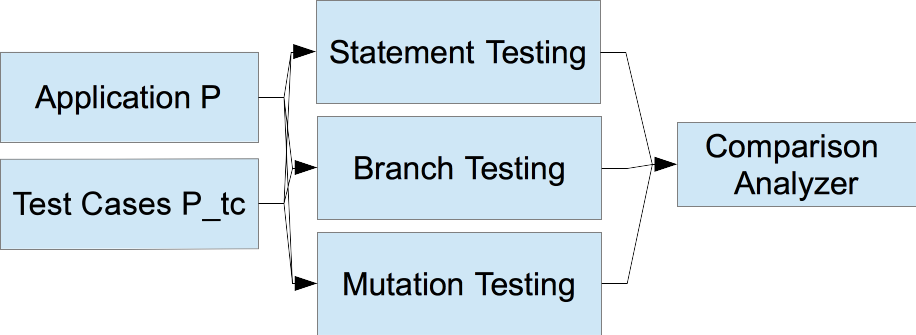
\includegraphics[scale=.4]{the_process.png}
\caption{The analysis approach.}
\label{fig:process}
\end{figure}
In this research, we compare the statement coverage, branch coverage, and mutation scores of programs that have been developed using TDD and other practices.  Our process can be seen in Figure~\ref{fig:process}.  Each application and its associated test suite is executed using a coverage analyzer tool and a mutation analyzer tool.  Given those results, we compare the coverage and mutation scores for different types of applications.

We expect that TDD approaches will exhibit high code coverage in terms of both statement and branch coverage, given the practices of TDD.  However, there is little known about the correlation between coverage and mutation score.  Applications that were developed using other methods are analyzed with the same tools.  We expect that coverage and mutation scores will be lower than those developed using TDD, especially for applications that are not developed within a large community or are not widely used.  

\section{Empirical Evaluation} % was proposed work section % change the numbering of the questions depends on the discussion tomorrow
In this paper, we compare the quality of TDD test suites to other those developed using more standard testing techniques. First, we observe the trends of quality in test suites that are written using TDD methodology. Next, we inspect the trends of quality when generating test suites using other development techniques. Then, we compare the quality of TDD test suites to other test suites developed using traditional techniques and observe the overall impact of code coverage criteria and mutation score criteria.  In summary, we analyze:
\squishlist
\item The relationship between coverage and mutation scores when applied to programs developed using TDD
\item The relationship between coverage and mutation scores when applied to programs developed using non-TDD methods
\squishend
Overall, we examine how traditional software testing  methodologies compare to newer testing methodologies, specifically test-driven-development (TDD) with regard to test suite quality.  We answer three key questions:

%Parahgraphs pattern: Questions then decomposed questions:
\textbf{RQ1:} What is the impact of TDD on test quality metrics?\\
In the way the TDD process is designed, it directly implies good coverage, as described in Sections~\ref{sec:background}. However, there is a little understanding in current research as to how  quality can be measured other than coverage. Another potential quality metric includes mutation metrics and, more specifically, mutation score. If we know that the code coverage is high in TDD applications, does that imply that the mutation score is also high, nearing 100\%? 
We have also observed that TDD applications claim high ``code coverage.'' In most work, it is unclear if code coverage refers to statement coverage, a lesser metric, or to branch coverage.  Thus, we also will also analyze if TDD test suites are creating high quality test suites in terms of both statement and branch coverage.

\textbf{RQ2:} What are the differences in the quality of test suites between TDD and other testing methodologies?\\
Once both quality metrics, coverage and mutation score, are taken into consideration, we next ask what qualities traditional test suites exhibit.  Traditional test suites are often developed in ad hoc fashions. Some may develop the tests in tandem with the writing of code, or the code may be written and then passed off to an external (away from the developer) Quality Assurance (QA) team for evaluation.  QA teams often test the code in an ad hoc, white-box, behaviorally or integration testing driven way.  For example, ``if I click this button, then I should arrive at this view and see these results.''  Tests written in this way account little for individual units of code or subtle integrations between components.\\
We examine traditionally created test suites for applications and evaluate the code coverage and mutation scores for each.  We hypothesize that the coverage and mutation scores will be lower than that of applications generated using TDD.  

\textbf{RQ3:} What are the trends in test quality metrics?\\
There are also some debatable questions that are related to the common quality metric, coverage. Coverage metrics, specifically those based on structure alone, are cheap to evaluate and thus, are most frequently used in industry.  For example, the avionics industry standard \texttt{DO-254} \cite{DO-254} demands that close to 100\% statement coverage be achieved.  The avionics industry standard \texttt{DO-178B} \cite{DO-178B} and automotive industry standard \texttt{IEC 61508} \cite{IEC61508} detail similar requirements. However, it is unclear if these metrics alone actually lead to higher fault finding ability.  

From our results from Q1 and Q2, we analyze the relationship between test suite quality metrics, code coverage and mutation score, across test methodologies that were used to develop the test suites. In our research, we answer two key questions: 1) What is the relationship between coverage and mutation score? 2) Does the comparison differ between different types of coverage? Finally, we discuss if it is enough to judge the test suite quality by traditional coverage metrics, or if other metrics, such as mutation score, should be considered.  Lastly, we discuss the differences observed between TDD generated applications versus traditionally generated applications.  %KJ- redundant and can be shortened a lot

\subsection{Experiment Design and Metrics}
In this section, we describe the experiment design including tools, metrics, and benchmarks that are used in our work, and then we explain the experiment evaluation.  

\subsubsection{Experiment design}
% Results
% the Big table of the whole results.
\begin{table*}[htbp]
\caption{Metrics of Case Study Applications}
\label{table:results}
\begin{tabular}{ c c c c c c c c c c c c c c c}
\hline
\textbf{} & \multicolumn{1}{l}{\rotatebox{270}{\textbf{Tyburn 1.1 }}} & \multicolumn{1}{l}{\rotatebox{270}{\textbf{Jbehave-core 3.9 }}} & \multicolumn{1}{l}{\rotatebox{270}{\textbf{Helium 0.1 }}} & \multicolumn{1}{l}{\rotatebox{270}{\textbf{Junit r4.11 }}} & \multicolumn{1}{l}{\rotatebox{270}{\textbf{Trove 3.0.3 }}} & \multicolumn{1}{l}{\rotatebox{270}{\textbf{Commons-lang 3.2 }}} & \multicolumn{1}{l}{\rotatebox{270}{\textbf{Commons-io 2.4 }}} & \multicolumn{1}{l}{\rotatebox{270}{\textbf{JDOM 2.0.6 }}} & \multicolumn{1}{l}{\rotatebox{270}{\textbf{Numerics4j 1.2 }}} & \multicolumn{1}{l}{\rotatebox{270}{\textbf{lavalamp }}} & \multicolumn{1}{l}{\rotatebox{270}{\textbf{netweaver }}} & \multicolumn{1}{l}{\rotatebox{270}{\textbf{Jaxen 1.1.6 }}} & \multicolumn{1}{l}{\rotatebox{270}{\textbf{twfbplayer }}} & \multicolumn{1}{l}{\rotatebox{270}{\textbf{JfreeChart }}} \\ \hline
\textbf{TDD ?} & YES & YES & YES & YES & NO & NO & NO & NO & NO & NO & NO & NO & NO & NO \\ \hline
\textbf{\#  Test classes excluded} & 0 & 8 & 0 & 43 & 0 & 0 & 1 & 0 & 0 & 1 & 0 & 0 & 0 & 6 \\ 
\textbf{\#  Generated mutants} & \textbf{229} & 3134 & 332 & 2097 & 72730 & 21974 & 6521 & 9448 & 3896 & \textbf{292} & 17237 & 7062 & 4175 & 70440 \\ \hline
\textbf{Statement coverage} & 92 & 81 & 94 & 48 & 7 & 94 & 88 & 95 & 99 & 91 & 16 & 79 & 15 & 57 \\ 
\textbf{Branch coverage} & 88 & 71 & 99 & 40 & 7 & 90 & 87 & 91 & 97 & 32 & 2 & 59 & 17 & 45 \\ 
\textbf{Mutation score} & 86 & 98 & 93 & 62 & 59 & 75 & 85 & 78 & 81 & 90 & 16 & 52 & 48 &  \\ \hline
\end{tabular}
\end{table*}

In our experiments, two sets of benchmarks will be evaluated using three key quality metrics: statement coverage, branch coverage, and mutation score.  In addition to these metrics, the benchmarks will be analyzed for their size, complexity, and other standard metrics.   Each metric will be evaluated using common tools. Experiments were executed using a 3rd Gen Intel Core i7-3770 processor 3.40GHz with 16GB DDR3 SDRAM.  

\subsubsection{Benchmarks}
	In our experiment, we have incorporated four TDD projects.  These benchmarks include  \texttt{Tyburn,Jbehave,Helium}  and \texttt{Junit}.  We also evaluate ten non-TDD projects including \texttt{trove, Commons Lang, JDOM, Commons IO, numerics4j,jaxen} and \texttt{JfreeChart} along with  \texttt{netweaver,lavalamp} and \texttt{twfbplayer} from SF100.
	
% + short description of the subject programs
 
% table of silent proprieties of the projects
\begin{table}[htbp]
\centering 
\caption{Subject Programs and their Silent Proprities}
\label{table:apps-proprities}
\begin{tabular}{ l l l l l }
\hline
\textbf{Subject Programs} & \multicolumn{1}{c}{\textbf{ Total java SLOC}} & \multicolumn{1}{c}{\textbf{Test SLOC}} & \multicolumn{1}{c}{\textbf{\# Test classes}} & \multicolumn{1}{c}{\textbf{CCN}} \\ \hline
\textbf{Tyburn 1.1} & 1209 & 655 & 32.0 & 1.33 \\
\textbf{Jbehave-core 3.9} & 17372 & 7646 & 207 & 1.57 \\
\textbf{Helium 0.1} & 2753 & 1735 & 50 & 1.95 \\
\textbf{Junit r4.11} & 12872 & 7825 & 690 & 1.72 \\
\textbf{Trove 3.0.3} & 12566 & 10486 & 91 & 2.24 \\
\textbf{Commons-lang 3.2} & 44457 & 28632 & 322 & 3.31 \\
\textbf{Commons-io 2.4} & 18057 & 12020 & 136 & 2.52 \\ 
\textbf{JDOM 2.0.6} & 27250 & 17010 & 284 & 2.51 \\ 
\textbf{Numerics4j 1.2} & 4596 & 2760 & 58 & 2.27 \\ 
\textbf{lavalamp} & 2383 & 1344 & 36 & 1.5 \\ 
\textbf{netweaver} & 19316 & 1363 & 41 & 2.82 \\ 
\textbf{Jaxen 1.1.6} & 14843 & 6415 & 102 & 3.21 \\
\textbf{twfbplayer} & 6382 & 862 & 2 & 1.72 \\ 
\textbf{JfreeChart} & 99154 & 32128 & 399 & 2.61 \\ \hline
\end{tabular}
\end{table}

We also calculate program and test attribute measurements to help us recognize the distinct trends in the code projects. We measure project characteristics including: total number of non-commented source code lines (Total java SLOC), number of non-commented source code lines of the test code (Test SLOC), cyclomatic complexity of the source code (CCN), and number of test classes (\# test classes).
 %, and test lines of code per source line of code (test-LOC/source-LOC). 
 These calculations are performed using JavaNCSS. JavaNCSS~\cite{leejavancss}  is a tool that can be used to count the non-commented lines of source code, as well as the McCabe cyclomatic complexity of the source code. The cyclomatic complexity~\cite{mccabe1976complexity} metric for software systems is adapted from the classical graph theoretical cyclomatic number and can be defined as the number of linearly independent paths in a program. Larger numbers of lines of code and increased complexity can imply poor design and greater challenges to thorough testing.

\subsubsection{Metrics}
We measure branch coverage, statement coverage, and mutation score on all projects.  Each of these metrics is described in Section~\ref{sec:background}.   Two main tools are used for these measurements: JaCOCO and MAJOR. JaCOCO \cite{hoffmann2007code} is an open source coverage library for Java, which has been created by the EclEmma team. JaCOCO reports code coverage analysis (.e.g. line, branch, instruction coverage) from the bytecode. MAJOR~\cite{just2011major} is a mutation testing and score tool.  The MAJOR mutation framework enables fundamental research on mutation testing as well as efficient mutation analysis of large software systems. The mutation framework provides the following three components:
\squishlist
\item Compiler-integrated mutator
\item Mutation analysis back-end for JUnit tests
\item A domain specific language to configure the mutation process
\squishend
       
 \begin{figure}[t!]
\centering
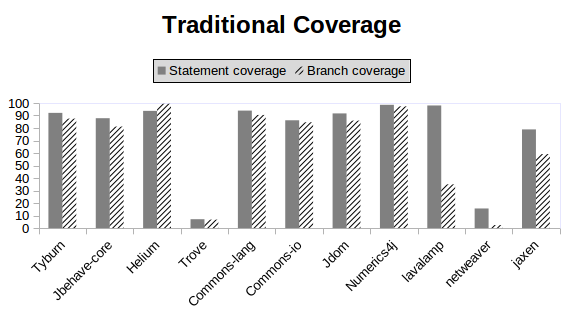
\includegraphics[scale=.4]{benchmark_coverage.png}
\caption{Statement and Branch coverage of benchmarks}
\label{fig:coverage}
\end{figure}
\begin{figure}[t!]
\centering
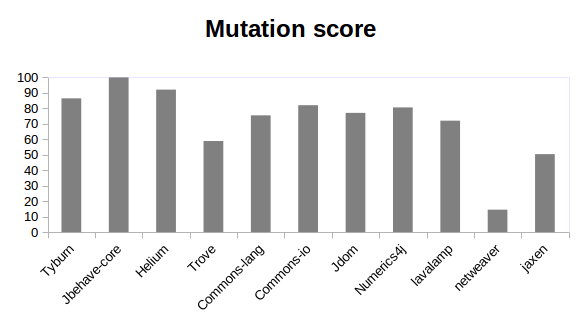
\includegraphics[scale=.4]{benchmark_mutation.png}
\caption{Mutation score of benchmarks with standard deviation}
\label{fig:mutations}
\end{figure}

\section{Threats To Validity}
The primary threats to validity of this research are internal and involve the benchmarks selected and the tools used.  We carefully selected TDD programs, \texttt{Tyburn, Jbehave} and \texttt{Helium}, from a list of TDD applications identified by Mark Levison~\cite{mlevinson:2008}.  Research into these applications reveal that they were developed using TDD practices based on documentation and code commits.  The other applications were also considered based on their documentation and code commits, and there is no indication that TDD practices were used.  Some programs, such as those included in Apache Commons, are well accepted and tested and thus could impact our results based on their high level of acceptance and support.  Other programs, such as those selected from the SF100, are less well-maintained or supported at this time, giving better evidence of ``normal'' programs.  In future work, a wider range of programs will be considered, including more TDD and non-TDD applications.

The tools used for coverage and mutation analysis also lead to a potential internal threat to validity.  Jacoco was used for all coverage analysis, and MAJOR was used for mutation analysis.  Jacoco is a well-founded tool for analyzing Java programs, based on Emma.  This is a standard tool for analyzing Java programs~\cite{jacoco:2014}.  MAJOR was developed by Ren\'{e} Just at the University of Washington~\cite{just2011using}.  This mutation tool has been built into the Java compiler. However, other options such as PIT~\cite{pitest:2014} could be used for comparison. 

\subsection{Results}
We evaluate the  . Also, we evaluate the statement coverage, branch code coverage, and mutation scores of all test suites of our selected benchmark programs, as can be seen in Table~\ref{table:results}.
  
  %HESSAH- why only one subsubsection? Should we break this up more?
  % Answer: I just break them into two susubsections for clarity. I didn't change anything. 
\subsubsection{TDD vs Traditional}
In this section we aim to answer these two questions:\\
\textbf{Q1:} What is the impact of TDD on other test quality metrics?\\
\textbf{Q2:} What are the differences in the quality of test suites between TDD and other testing methodologies?

%answer to Q1
Figure~\ref{fig:coverage} illustrates the statement and branch coverage for each program including programs of both groups the TDD and the non-TDD programs. From these results, we observe that the TDD applications (\texttt{Tyburn, Jbehave, and Helium}) exhibit high branch coverage of more than 80\% and statement coverage of more than 88\%.  Several of the non-TDD applications also exhibit very high branch and coverage scores, namely \texttt{Commons-lang, Commons-io, Jdom,} and \texttt{Numerics4j}.  We suspect that these higher coverage metrics are due to the fact that these four applications are under active development in large communities that have high standards for acceptance of new features.  \texttt{Trove} has a high Test-LOC/Source-LOC because nearly all testing effort is focused on one significant package.  The other packages are mostly ignored, thus yielding low coverage results when the entire application is considered.  %HESSAH- Why would statement be lower for Helium?  If this is byte code based, this shouldn't be possible... need to explain.  From the table, I think you mixed up the two numbers for Helium? % Answer: Thanks very good catch !! (RESOLVED)

We next measured the mutation scores using MAJOR~\cite{just2012redundant, just2012usingnon-redundant, just2011major}. In Figure~\ref{fig:mutations}, we visualise the results of all benchmarks. %KRISTEN- Fix this- talked to Jesh and it's not a GA-- really confused about why we need standard deviation %HESSAH- Can you explain why the mutation score for lava lamp has such a high standard deviation? % Answer: there was a webRunTest that sometimes gets run and the other times it doesn't.  Once that test gets run the mutation score goes higher. (NEED INVESTIGATION) 
For the TDD applications under consideration,  \texttt{Tyburn} (non-TDD) exhibited the lowest mutation score at 86\% whereas  \texttt{Jbehave} (TDD) had a score of 100\%. On the other hand, the mutation score in non-TDD programs ranged from 15\% in \texttt{Netweaver} to 82\% for \texttt{commons-io}. Moreover, from Figures~ \ref{fig:mutations} and~\ref{fig:coverage}), we see that the quality of tests developed using TDD is not only high in terms of statement and branch coverage but also in terms of the mutation score metric.  

% following is the answer to Q2
%HESSAH- Need to reference the figures!
Then, we explored if TDD and non-TDD applications %and associated test suites 
are significantly different in term of their tests. %HESSAH- in terms of mutation score or coverage? I'm confused. Which two groups? % Answer: I am adding this sentence to introduce our answer to Q2 - in term of both test qualitymetrics mutation and coverage. I modifyied the sentence (RESOLVED)
To show this, we compare the means of the two groups using a two sample t-test for the normal groups and a non-parametric test on the data that the normality test shows as not normal. Thus, we first test the normality of our data using the Shapiro-Wilk test. % KRISTEN: I added the next sentence. Look at the grammer please
We explored the normality of two variables: branch coverage and mutation score. We test both the mutation score metric and the branch coverage metric assuming that branch coverage will already includes statement coverage~\cite{steve2011Code}.  

As show in Figure~\ref{table:Results of normality test}, specifically the normality indicator p-value in the last column, the results of the normality test shows that the data is normal for both groups,TDD and non-TDD, except in the mutation score of non-TDD group which was 0.029,because the value is less than 0.05, it indicates that the there is an evidence that the data tested are not from a normally distributed population. % HESSAH- need to clarify this sentence.  How is it normal for both groups? Again, I'm not understanding something here % Answer: I added a sentence above and clerify the "two groups" (RESOLVED)
\begin{figure}[t!]
\centering
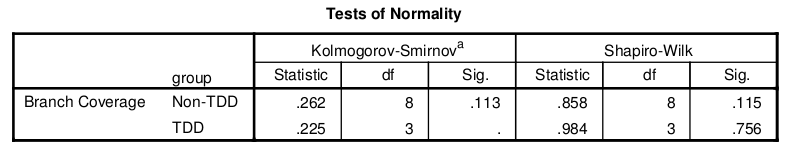
\includegraphics[scale=.32]{test_of_normality_Branch.png}
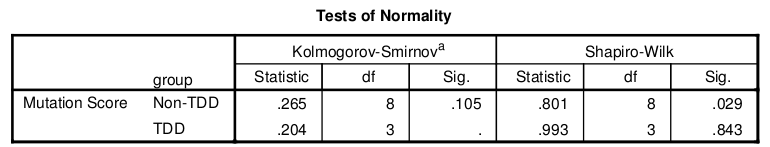
\includegraphics[scale=.33]{test_of_normality_mutation.png}
\caption{Results of normality test}
\label{table:Results of normality test}
\end{figure}
\begin{figure}[t!]
\centering
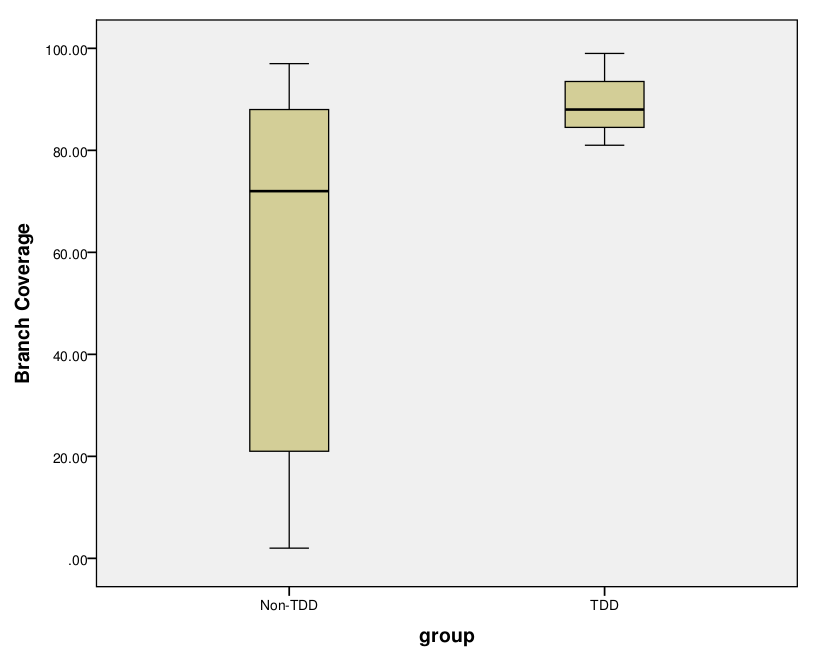
\includegraphics[scale=.3]{groups_branch.png}
\caption{Differences in branch coverage between TDD and Non-TDD applications }
\label{figure:groups_branch}
\centering
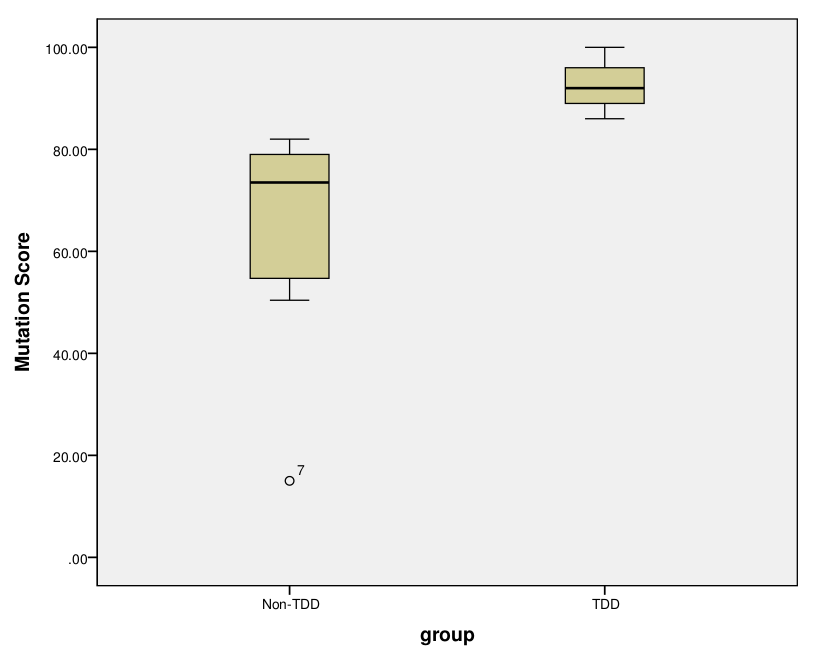
\includegraphics[scale=.3]{groups_mutation.png}
\caption{Differences in mutation score between TDD and Non-TDD applications}
\label{figure:groups_mutation}
\end{figure}

Next, according to the normality test, we compare the means of the two groups using either a "two sample t-test" for the normal data or "non-parametric test" for the data that is not normally distributed. Comparing the two groups of applications in terms of the branch coverage metric, the p-value was 0.059 which is not significant, but is approaching statistically significant results. Therefore, we can speculate that with more TDD programs we might be able to conclude a statistically significant difference between the application groups, where the TDD group has higher branch coverage than the non-TDD group. On the other hand, the Shapiro-Wilk test shows that the mutation score of non-TDD group is not normally distributed. Therefore, to compare the means, we used a non-parametric two-Sample test on this data. Namely, we applied the non-parametric independent samples in a Mann-Whitney U test and learned that the results of this tests had a p-value equal to 0.012. Therefore, we can conclude that the mutation score of the two groups are significantly different, where the TDD approach scored higher than the non-TDD approaches.

%HESSAH- Where do you reference these?  NEED TO INCLUDE % Answer: I didn't add explanation to these graphs yet (NEED FIX)
% add graphs that visually compares the two groups. ( one for branch the other for mutation score ) 
Figures~\ref{figure:groups_branch} and~\ref{figure:groups_mutation} demonstrate the relationship between mutation score and the two coverage types. As seen in the first box plot in Figure~\ref{figure:groups_branch}, the mean, the standard deviation, and the confidence interval for TDD group on branch coverage is (M=89.33, SD=9.07 , CI 95\%: 66.79 to 111.87) while the values for the non-TDD group are (M=57.63, SD=38.40, CI 95\%: 25.52 to 89.73). The second plot, shown in Figure~\ref{figure:groups_mutation}, demonstrates that the TDD group scores higher based on mutation score (M=92.67, SD=7.02 , CI 95\%: 75.22 to 110.11) than the non-TDD group (M=63.93, SD=22.61, CI 95\%: 45.03 to 82.83), where $M, SD,$ and $CI$ stand for the mean, standard deviation, and confidence interval respectively.    


\subsubsection {Mutation Score versus Coverage}
We use the correlation coefficient Pearson's r test to analyze the strength of the correlation between the metrics. The correlation coefficient is a value that ranges between $-1 \leq r \leq 1$. In our results shown in Table~\ref{table:benchmark_relation_mutationScoreWithBranch}, the correlation $r$ value for mutation score is .791 with branch coverage and 0.731 with statement coverage. The correlation coefficient indicates the existence of a relationship between these test quality metrics. Also, when analyzing the statistical significance of the resulting correlation, p-value of the correlation with branch coverage is 0.004 and it is 0.0.011 for the correlation with statement coverage (shown in the second row of Table~\ref{table:benchmark_relation_mutationScoreWithBranch}). Therefore, the correlation is statistically significant because the p-value is below 0.05. %HESSAH- we need to revise this last sentence- I'm not confident enough to rewrite it myself. % Answer: (RESOLVED) take a look.

\begin{table*}[t!]
\caption{The relationship between Mutation score metric with Statement and Branch coverage}
\label{table:benchmark_relation_mutationScoreWithBranch}
\centering
\begin{tabular}{|l l|r|r|}
\hline
 &  & \multicolumn{1}{c|}{Branch Coverage} & \multicolumn{1}{c|}{Statement Coverage} \\ \hline
\multicolumn{ 1}{|c}{Mutation Score} & Pearson Correlation & .791** & 0.731* \\
\multicolumn{ 1}{|l}{} & Sig. (2-tailed) & 0.004 & 0.011 \\
\multicolumn{ 1}{|l}{} & N & 11 & 11 \\ \hline
\multicolumn{ 4}{|l|}{*. Correlation is significant at the 0.05 level (2-tailed)}\\
**. Correlation is significant at the 0.01 level (2-tailed). \\ \hline
\end{tabular}
\end{table*}


We also calculate the coefficient of determination R-squared. As shown in Figure~\ref{figure:benchmark_relation_mutationStatment}, the mutation score is dependent on the statement coverage, and it can be predicted based on the statement coverage, the independent variable. As visualized in the figure, the rounded R-squared value of 0.54 indicates an existent relationship between the statement coverage and the mutation score, where almost 54\% of the variation in statement coverage can be explained by the variation in mutation score.

\begin{figure}[t!]
\centering
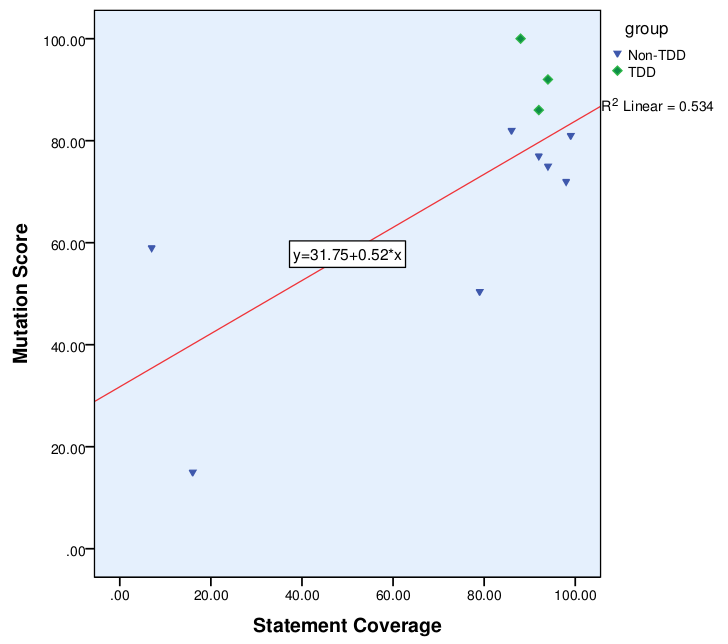
\includegraphics[scale=.3]{benchmark_relation_mutationStatment.png}
\caption{The relationship between mutation score and statement coverage.}
\label{figure:benchmark_relation_mutationStatment}
\end{figure}
 
Similarly, Figure~\ref{figure:benchmark_relation_mutationBranch}  reflects a relation where the coefficient of determination is 0.62. Thus, 62\% of the programs that had high branch coverage also achieved a high mutation score.

\begin{figure}[t!]
\centering
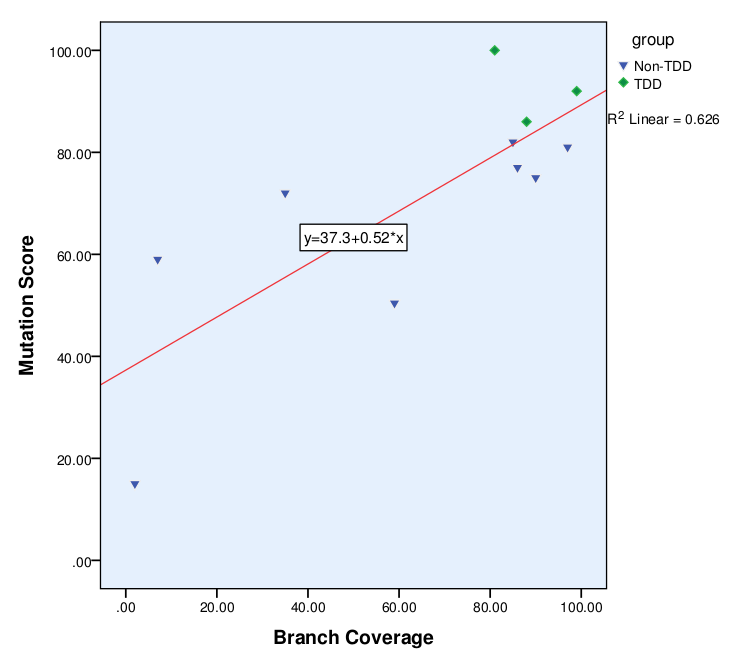
\includegraphics[scale=.3]{benchmark_relation_mutationBranch.png}
\caption{The Relationship between mutation score and branch coverage}
\label{figure:benchmark_relation_mutationBranch}
\end{figure}

Despite the fact that 62\% of the programs can be explained by the relationship between mutation score and branch coverage,  36\% of the programs in our study cannot be reliably explained with regard to this relation. %The correlation between statement coverage cannot be explained by the observed branch and mutation score correlation. 
To illustrate, in \texttt{lavalamp}  branch coverage scores were 35\% whereas the mutation score reaches 75\%. We believe this was because the statement coverage of this program was as high as 98\%. Other programs cannot be explained by either by branch or statement coverage. For example, in \texttt{common-lang} the branch coverage of \texttt{common-lang} is equal to 90\% and the statement coverage is 94\%. However, its mutation score is 75\%. 

\section{Discussion}
% trends in TDD 
In TDD, we found a trend between test-LOC per Source-Line of Code with high branch coverage and statement coverage. In other words, as more tests are written in TDD, branch and the statement coverage improve. The R-squared value is a linear relationship of 0.89 corresponding to statement coverage and 0.99 to branch coverage. This indicates that TDD programs tend to focus test writing based on code branches. It is known that executing every branch executes every statement as well unless there is a break or a jump \cite{hoffmann2007code}. Therefore, as a consequence of the high branch coverage in TDD programs, the statement coverage and the mutation score of TDD programs is also high.

% discuss the relationship between mutation and coverage
Mutation score metrics have a relationship not only with branch coverage but also with statement coverage. Both statement and branch coverage will complimentarily predict mutation score. Looking at \texttt{Lavalamp} as an example,the statement coverage is 98\%, the branch coverage is 35\% and the mutation score is 72\%. Despite the low branch coverage of \texttt{LavaLamp}, which was 35\%, the mutation score of \texttt{Lavalamp} is 72\%, which is not low. This could at first glance bring up a question about the relationship between the mutation score and the branch coverage. However, we show in our results that the mutation score can be predicted from both branch and statement coverage in most cases. In this case, the non-killed mutants of \texttt{Lavalamp} were due to the uncovered branches that have not been tested.     

% discuss general trends 
Our results conclude that writing more test cases does not necessary ensure good test suite quality on both metrics. We found no relation between Test-LOC/source-LOC. The coefficient of determination of Test-LOC with the mutation score coverage was 0.02 and was 0.05 with branch coverage. Writing more tests could give little extra value, such as in \texttt{trove} where the TLOC/SLOC is the highest among the projects as seen in Table~\ref{table:results}, but the tests did not reflect a very high mutation score or coverage because most of \texttt{trove}'s  tests were written for one or two modules of the source, leaving the other modules not tested.  Also, \texttt{Lavalamp} exhibited low branch coverage at 35\% while its Test-LOC/source-LOC is not low. One possible explanation is that most of the tests were written to cover the statements, not the branches.  There is approximately one line of test per line of source code. However as we discussed in Section~\ref{sec:background}, if the tests cover 100\% of the lines, that does not indicate anything about branch coverage. When most of the branches of a program are covered, its statements are mostly covered.

We also want to know if the program size in our experiments impacts the mutation score that we are getting for each program. We found that larger sized programs do not correlate  to lower mutation scores. Only 24\% of applications can be explained by this connection. For example, \texttt{netweaver} falls under one of the 24\% of programs in our benchmarks that can explained from this relation. However, this relation also is questionable since the most accurate interpretation of the low mutation score of \texttt{netweaver} is not because of the program size but because \texttt{netweaver} was not tested enough according to our calculated test-line-of-code to source-line-of code metric, which was only 0.1 for this project.

\section{Conclusion and Future Work}
In this paper, we performed a test suite quality based evaluation for the TDD testing process. We demonstrated the effect of TDD practices on test suite quality and compared that to other testing methodologies. Test suite quality is measured based on branch and statement coverage compared to mutation scores.  Finally, we discuss the correlation between code coverage quality and mutation scores.

We have quantitatively evaluated Test-Driven-Development (TDD) by applying test quality metrics to three open source projects. Our study gives an evidence that the Test-driven development is indeed an effective approach for writing high quality tests to support the maintenance and evolution of software. 

We analyzed differences in test suite quality between TDD groups and other in-use development techniques. The difference between the TDD and non-TDD groups is approaching significance on branch coverage, ($t=2.179, p=0.059$). The mutation score metric of the TDD application group is significantly different from the non-TDD group, as shown by the results of the Mann-Whitney U test ($p = .012$).

  %HESSAH- what's CI? % it is the "Confidence Interval". In the yellow small paper from your discussion with Emily shy would see it. ( MIGHT NEED ADDITIONAL EXPLANATION)
Finally, we evaluated the correlation between code coverage quality and mutation scores. We discovered that mutation scores are significantly correlated to both types of coverage quality. The relationship between mutation scores and branch coverage was significant ($r = 0.79, p < 0.05$), as  was the relationship between mutation scores and  statement coverage ($r = 0.73, p < 0.05$). We determined that the mutation score often can be predicted from both traditional metrics, statement and branch coverage.  Both metrics,when examined together, indicate a higher likelihood to kill mutants. 64\% of the programs' mutation scores can be anticipated based on branch coverage.  A lower percentage of 54\% of the programs' mutation scores can be predicted by the statement coverage.

Some of the programs in our experiment cannot be predicted either by branch or statement coverage. Therefore, there are factors other than the branch coverage and statement coverage that impact mutation score. Those factors are not included in our study and are left for future research to explain program cases such as \texttt{Jbehave} and \texttt{common-lang} programs. %In \texttt{Jbehave} the rounded mutation score is the highest at 100\%  although the branch coverage is below 90\%. In a contrary example, the branch coverage of \texttt{common-lang} is equal to 90\% while its mutation score is 75\%. 
In future work, we will analyze such programs and their associated tests further and incorporate a larger range of TDD and non-TDD developed applications.

\section*{Acknowledgment}
The authors would like to thank Dr. Ren\'{e} Just, the developer of MAJOR, which we used as our mutation analysis tool, for giving us access to the tool and for his help and guidance in its usage, and Dr. Gregory M. Kapfhammer for his guidance and help in the tools and research for this project.

\bibliographystyle{plain}
\bibliography{proposal_bib}

\end{document}

% add my work is different in this way and that to Related Work section
